\documentclass[conference]{IEEEtran}
\usepackage{cite}
\usepackage{amsmath,amssymb,amsfonts}
\usepackage{graphicx}
\usepackage{textcomp}
\usepackage{xcolor}
\usepackage{booktabs}

\begin{document}

\title{VeriSight: Consistency-Gated Multimodal Verification and Calibrated Explainability Across Video, Audio, Image, and Multilingual Text}

\author{\IEEEauthorblockN{Piyush Punera (S24CSEU1772), Vaibhav Pant (S24CSE1765), Ayush Jain (S24CSEU1752),\\
Vinit Jha (S24CSEU1753), and Nimish Jain (S24CSEU1751)}
\IEEEauthorblockA{\textit{SCSET, Bennett University, Greater Noida, India}}}

\maketitle

\begin{abstract}
Single-modality deepfake detectors fail regularly when attackers alter only one stream—for example, pairing authentic camera footage with cloned speech or attaching misleading text claims to unedited images. We present VeriSight, a three-layer multimodal verification system built and evaluated across two 6\,GB RTX~4050 workstations for video, audio, photographic images, and English, Hindi, and Hinglish text. Rather than training heavy backbones from scratch, we freeze EfficientNet-B0, wav2vec2-XLS-R-300M, and XLM-RoBERTa-base as feature extractors and train compact 256-dimensional projection adapters (<1.4\,MB each) alongside a custom Consistency-Gated Fusion network with 20\% modality dropout. Cross-modal checks track mouth-motion versus audio RMS correlation (AV-Sync) and Whisper ASR alignment against captions. Across three seeds, Consistency-Gated Fusion reaches 0.7318 F1 and 0.9359 ROC-AUC, beating Concat MLP (0.4571 F1) and Cross-Attention (0.4402 F1) while lowering ECE to 0.1382 after temperature scaling ($T = 1.6069$). We also report failure modes observed in practice: CLIP identity overfitting on Celeb-DF v2, Fakeddit label inversion, compressed-portrait false positives from SDXL-only diffusion detectors, and audio domain shift from 0.9975 ROC-AUC on ASVspoof 2019 LA down to 0.5757 on unseen out-of-domain speech.
\end{abstract}

\begin{IEEEkeywords}
Multimodal deepfake detection, consistency-gated fusion, cross-lingual Hindi/Hinglish forensics, temperature scaling, Grad-CAM.
\end{IEEEkeywords}

\section{Introduction}
Most deepfake detectors treat manipulation as a single-stream classification problem: a face-swap model inspects cropped video frames, an acoustic classifier scores speech segments, and a text classifier checks prose style. In real social-media feeds, manipulation rarely stays isolated to one signal. A real news clip can carry a fabricated voiceover, a compressed WhatsApp screenshot can trip an image diffusion detector, and misleading Hindi or Romanized Hinglish forwards often bypass English-only text classifiers.

Deploying deepfake detection in an academic or consumer setting also exposes three engineering constraints that benchmark papers often overlook. First, 6\,GB laptop GPUs cannot fine-tune 300M-parameter audio or multilingual transformers end-to-end without heavy memory offloading. Second, binary forced-choice classifiers (\texttt{REAL} vs.\ \texttt{FAKE}) produce overconfident errors on compressed or out-of-domain media. Third, raw subword attributions and ungrounded scores give human reviewers no clear reason to trust a verdict.

We built VeriSight to address three practical gaps identified across recent multimodal forensics literature [1]--[3]:
\begin{enumerate}
\item \textbf{Cross-modal contradictions:} Combining visual, acoustic, and textual streams through learned consistency signals rather than naive score averaging or feature concatenation [9], [14].
\item \textbf{Multilingual and noisy human text:} Handling English, Devanagari Hindi, and Romanized Hinglish without misclassifying casual human typos or regional vocabulary as machine-generated text [16].
\item \textbf{Calibrated abstention:} Returning an explicit \texttt{UNCERTAIN} verdict under high predictive entropy instead of forcing low-confidence binary guesses [3], [11].
\end{enumerate}

Unlike systems that depend on large multimodal LLMs at inference time [6], [7], VeriSight runs locally on consumer hardware (CPU inference under 1\,s after warmup; adapter training inside 6\,GB VRAM) and exposes every intermediate score, Grad-CAM overlay, and whole-word token weight in an interactive verification workstation.

\section{Related Work}
Early visual forgery benchmarks such as FaceForensics++ [17] and Celeb-DF [15] established that frame-level CNNs degrade sharply under video compression and cross-identity evaluation, while Face X-Ray [18] and Self-Blended Images [19] showed that focusing on blending boundaries improves generalization across unseen face-swap generators. Subsequent audio-visual datasets including FakeAVCeleb [12], DFDC [20], and AV-Deepfake1M [4] showed that pairing unmanipulated video with synthetic speech defeats unimodal face detectors. Recent joint architectures—AVoiD-DF [7], AVFF [5], and LipForensics [13]—demonstrate that lip-motion correspondence and cross-modal feature alignment catch audio-visual tampering.

In image and text forensics, UnivFD [8] and Cozzolino et al. [6] showed that frozen CLIP spaces generalize across diffusion families better than pixel-level classifiers, while FakeShield [1] highlighted the need for spatial localization and deletion-faithfulness audits. On the audio side, AASIST [10] and Mueller et al. [11] documented severe performance drops when acoustic spoof detectors face out-of-domain (OOD) vocoders. For multimodal text, r/Fakeddit [16] and MMFakeBench [2] exposed the prevalence of out-of-context captions, and CAFE [9] introduced cross-modal ambiguity estimation. VeriSight integrates these findings into a unified, resource-constrained three-layer pipeline with Hindi and Hinglish support.

\section{System Architecture and Formulation}
VeriSight processes media across three sequential layers: unimodal forensic encoding (Layer~1), cross-modal consistency measurement (Layer~2), and consistency-gated fusion with post-hoc calibration (Layer~3).

\subsection{Layer 1: Frozen Backbones and Lightweight Adapters}
Freezing large foundation models keeps trainable adapter checkpoints between 0.53\,MB and 1.32\,MB, allowing distributed training across two RTX~4050 laptops via standard Git synchronization:
\begin{itemize}
\item \textbf{Visual Branch (\texttt{VisualV2Detector}):} Extracts spatial artifact features from frozen \texttt{efficientnet\_b0} followed by a trainable 256-d LayerNorm-GELU projection (460,289 trainable parameters) and $224\times224$ Grad-CAM spatial saliency. Given feature maps $A^k \in \mathbb{R}^{H'\times W'}$ from the final convolutional stage and class logit $y_v$, Grad-CAM weights $\alpha_k = \frac{1}{H'W'}\sum_{i,j}\frac{\partial y_v}{\partial A^k_{i,j}}$ produce normalized spatial heatmaps $\text{ReLU}(\sum_k \alpha_k A^k)$. Live frame and portrait inspection pairs this spatial head with \texttt{deepfakeguard-v2} ONNX face-crop inference (18\% margin, horizontal-flip TTA, minimum 3/8 tracked faces with MTCNN confidence $\ge 0.92$).
\item \textbf{Audio Branch (\texttt{AudioV2Detector}):} Extracts frame-level hidden states $H = [h_1, \dots, h_T]$ from frozen \texttt{wav2vec2-xls-r-300m} over 16\,kHz mono speech windows ($\ge 0.5$\,s active energy), followed by learned temporal attention pooling:
\begin{equation}
\alpha_t = \frac{\exp(w_2^\top \tanh(W_1 h_t))}{\sum_{j=1}^{T}\exp(w_2^\top \tanh(W_1 h_j))}, \quad \bar{h} = \sum_{t=1}^{T}\alpha_t h_t
\end{equation}
and an L2-normalized 256-d projection $e_a = \text{norm}(\text{GELU}(\text{LN}(W_a \bar{h})))$.
\item \textbf{Text Branch (\texttt{TextV2Detector}):} Uses frozen \texttt{xlm-roberta-base} with masked token-attention pooling (246,914 trainable parameters) and a 256-d adapter. During inference, SentencePiece subword pieces starting without the \texttt{\_} word-boundary prefix are merged into complete words with summed attention weights so attributions remain readable in English, Hindi, and Hinglish.
\end{itemize}

\subsection{Layer 2: Cross-Modal Consistency Engine}
Given L2-normalized embeddings $(e_v, e_a, e_t)$, Layer~2 constructs a three-element consistency vector $c = [c_{vt}, c_{at}, c_{av}] \in [0, 1]^3$, mapping cosine similarity into $[0,1]$ via $(\cos(e_i, e_j) + 1)/2$. Missing streams default to neutral $0.50$ so downstream layers never fail on silent videos or text-free uploads. For video files containing tracked faces and decodable audio, \texttt{AVSyncDetector} samples frames at 8\,fps, crops the lower mouth region, extracts frame-to-frame motion energy $m(t)$, and computes Pearson correlation $r$ against the 16\,kHz RMS/spectral envelope $a(t)$:
\begin{equation}
c_{av} = \frac{1 + \text{corr}(m(t), a(t))}{2} \in [0, 1]
\end{equation}
Scores below $0.30$ trigger an audio-visual contradiction warning. When user captions or subtitles are provided, \texttt{faster-whisper-tiny} transcribes spoken speech for lexical and semantic comparison.

\subsection{Layer 3: Consistency-Gated Fusion and Calibration}
Our proposed \texttt{ConsistencyGatedFusion} module concatenates modality embeddings, $c$, and a binary availability mask $m \in \{0,1\}^3$ into a gating MLP that outputs masked softmax weights:
\begin{equation}
g = \text{softmax}\big(\text{mask}(\text{MLP}_g([e_v, e_a, e_t, c, m]), m)\big) \in \Delta^2
\end{equation}
During training, each modality is randomly dropped with probability $p = 0.20$ while guaranteeing at least one active stream per sample. The gated representation $e_{\text{fused}} = g_v e_v + g_a e_a + g_t e_t$ is concatenated with a 32-d projection of $c$ before binary logit prediction $z$. Post-hoc temperature scaling ($z_{\text{cal}} = z / T$, with $T$ fit via L-BFGS on validation logits) and binary predictive entropy $H(p) = -p\log_2 p - (1-p)\log_2(1-p)$ govern three-way abstention (\texttt{REAL}, \texttt{FAKE}, \texttt{UNCERTAIN}).

\subsection{Full-Stack Inference Pipeline and Workstation UI}
We expose the pipeline via FastAPI endpoints (\texttt{/api/predict}, \texttt{/api/predict/audio}, \texttt{/api/predict/image}, \texttt{/api/predict/text}, and \texttt{/api/v2/metrics}) backed by PyAV and FFmpeg media decoding. A React and TypeScript forensic interface renders 1-click demo presets, Grad-CAM face overlays, whole-word token chips, cross-modal contradiction alerts, and live benchmark charts.

\section{Datasets and Empirical Engineering Fixes}
Table~\ref{tab:datasets} summarizes all datasets used for training and evaluation. During live deployment testing, we observed four concrete failure modes and resolved each without leaking evaluation splits:

\begin{table}[htbp]
\caption{Datasets and Splits Used in VeriSight}
\label{tab:datasets}
\centering
\begin{tabular}{@{}llll@{}}
\toprule
\textbf{Modality} & \textbf{Dataset} & \textbf{Split} & \textbf{Notes} \\
\midrule
Video & Celeb-DF v2 & 302 / 38 / 60 & Identity-disjoint \\
Audio & ASVspoof 2019 LA & Dev + 71,237 eval & In-domain TTS/VC \\
Audio OOD & WaveFake / Eval & 600 clips & Unseen codecs \\
Text (EN) & HC3 + Fakeddit & 8,781 in train & Polarity fixed \\
Text (HI/HG) & HinglishBench & 1,482 tr / 136 te & Disjoint (rows 65+) \\
\bottomrule
\end{tabular}
\end{table}

\begin{enumerate}
\item \textbf{Fakeddit Label Polarity:} In Fakeddit's \texttt{2\_way\_label} schema, \texttt{1} denotes real and \texttt{0} denotes fake—opposite to our convention. Flipping labels via $1 - y$ on six text-focused subreddits eliminated inverted English predictions.
\item \textbf{CLIP Identity Overfitting:} Enabling CLIP ViT-B/32 alongside EfficientNet-B0 yielded 0.9562 validation AUC on Celeb-DF v2 but collapsed to 0.4921 ROC-AUC on identity-disjoint test clips because the 768-d semantic vector memorized training identities. Disabling CLIP in the visual adapter restored cross-identity generalization (0.9226 val AUC, 0.6380 standalone test AUC, 0.9359 fused AUC).
\item \textbf{Multilingual Coverage and Typo Protection:} Training purely on English caused real Hindi weather bulletins to score 77.5\% fake while Hinglish RBI hoax forwards scored 17.0\%. Adding 1,482 disjoint Hindi/Hinglish samples (HinglishBench rows 65--308 plus curated journalism and scam pairs, upsampled $3\times$) pushed cross-lingual test accuracy to 99.26\% (0.9927 F1). For English inputs, a dual-detector consensus between \texttt{XLM-R} and \texttt{roberta-base-ai-text-detection-v1} applies human-protective weighting ($0.75\min + 0.25\max$) when either detector scores $<0.15$ and the other $<0.85$, preventing false flags on human typos (78.8\% \texttt{REAL} vs.\ 98.6\% \texttt{FAKE} on GPT prose).
\item \textbf{Compressed Portrait Hybrid Routing:} \texttt{Organika/sdxl-detector} flagged compressed WhatsApp JPEGs and PNG screenshots of real faces at $>99\%$ fake. Branching \texttt{AI-Image Check} through face detection ($0.65\text{ Face-Crop} + 0.20\text{ EffNet-B0} + 0.15\text{ Diffusion}$) recovered real portraits (87.8\% \texttt{REAL} on webcam photos, 68.6\% \texttt{REAL} on group selfies) while retaining 83.0\%--84.5\% \texttt{FAKE} detection on synthetic room renders.
\end{enumerate}

\section{Experimental Evaluation}
All multimodal fusion experiments were evaluated across three random seeds (42, 123, 2025) on aligned embeddings from Laptop~1 (Visual/Text) and Laptop~2 (Audio).

\begin{table}[htbp]
\caption{Unimodal and Cross-Lingual Branch Performance (Exp~1)}
\label{tab:unimodal}
\centering
\begin{tabular}{@{}lccc@{}}
\toprule
\textbf{Branch / Evaluation Set} & \textbf{Acc} & \textbf{F1} & \textbf{ROC-AUC} \\
\midrule
Visual (\texttt{EffNet-B0}, Celeb-DF Val) & 0.8421 & 0.7273 & 0.9226 \\
Audio (\texttt{XLS-R}, ASVspoof 71,237) & 0.9685 & 0.9821 & 0.9975 \\
Audio OOD (WaveFake / Eval 600) & 0.5283 & 0.6222 & 0.5757 \\
Text EN (HC3 + Fakeddit Val) & 0.9564 & 0.9421 & 0.9889 \\
Text Cross-Lingual (HI/HG 136) & 0.9926 & 0.9927 & --- \\
\bottomrule
\end{tabular}
\end{table}

\begin{table}[htbp]
\caption{Three-Seed Fusion Comparison and Ablation (Exp~2 \& Exp~4)}
\label{tab:fusion}
\centering
\begin{tabular}{@{}lccc@{}}
\toprule
\textbf{Strategy / Ablation} & \textbf{F1 Score} & \textbf{ROC-AUC} & \textbf{ECE $\downarrow$} \\
\midrule
Concat + MLP (Baseline) & $0.4571 \pm 0.000$ & 0.8318 & 0.3237 \\
Cross-Attention & $0.4402 \pm 0.057$ & 0.8360 & 0.3260 \\
\textbf{Consistency-Gated (Ours)} & $\mathbf{0.7318 \pm 0.058}$ & \textbf{0.9359} & \textbf{0.1800} \\
\midrule
Calibrated ($T = 1.6069$) & 0.7442 & 0.9152 & \textbf{0.1382} \\
\midrule
Ablation: All Present & 0.7727 & 0.9389 & 0.1534 \\
Ablation: Drop Audio & 0.6500 & 0.8812 & 0.2286 \\
Ablation: Drop Text & 0.7442 & 0.8450 & 0.1888 \\
Ablation: Drop Visual & 0.8571 & 0.9457 & 0.1231 \\
\bottomrule
\end{tabular}
\end{table}

Table~\ref{tab:fusion} shows that Consistency-Gated Fusion outperforms Concat MLP by +0.2747 F1 and reduces calibration error by 44\% before temperature scaling. After fitting $T = 1.6069$ on validation logits, ECE drops to 0.1382 with an abstention rate of 18.33\%, and masking top attributed features reduces model confidence by 0.0907 (Deletion Faithfulness).

\begin{table}[htbp]
\caption{Experiment 3 Compression and Noise Stress Results}
\label{tab:stress}
\centering
\begin{tabular}{@{}llccc@{}}
\toprule
\textbf{Stress Type} & \textbf{Level} & \textbf{Acc} & \textbf{F1} & \textbf{AUC} \\
\midrule
Audio Noise (600) & SNR 20\,dB & 0.7517 & 0.7732 & 0.8528 \\
Audio Noise (600) & SNR 10\,dB & 0.7800 & 0.7708 & 0.8602 \\
Audio Noise (600) & SNR 5\,dB & 0.7550 & 0.7721 & 0.8437 \\
H.264 Video (40) & CRF 23 / 32 / 40 & 0.7500 & 0.7826 & 0.8075 \\
\bottomrule
\end{tabular}
\end{table}

\begin{figure}[htbp]
\centering
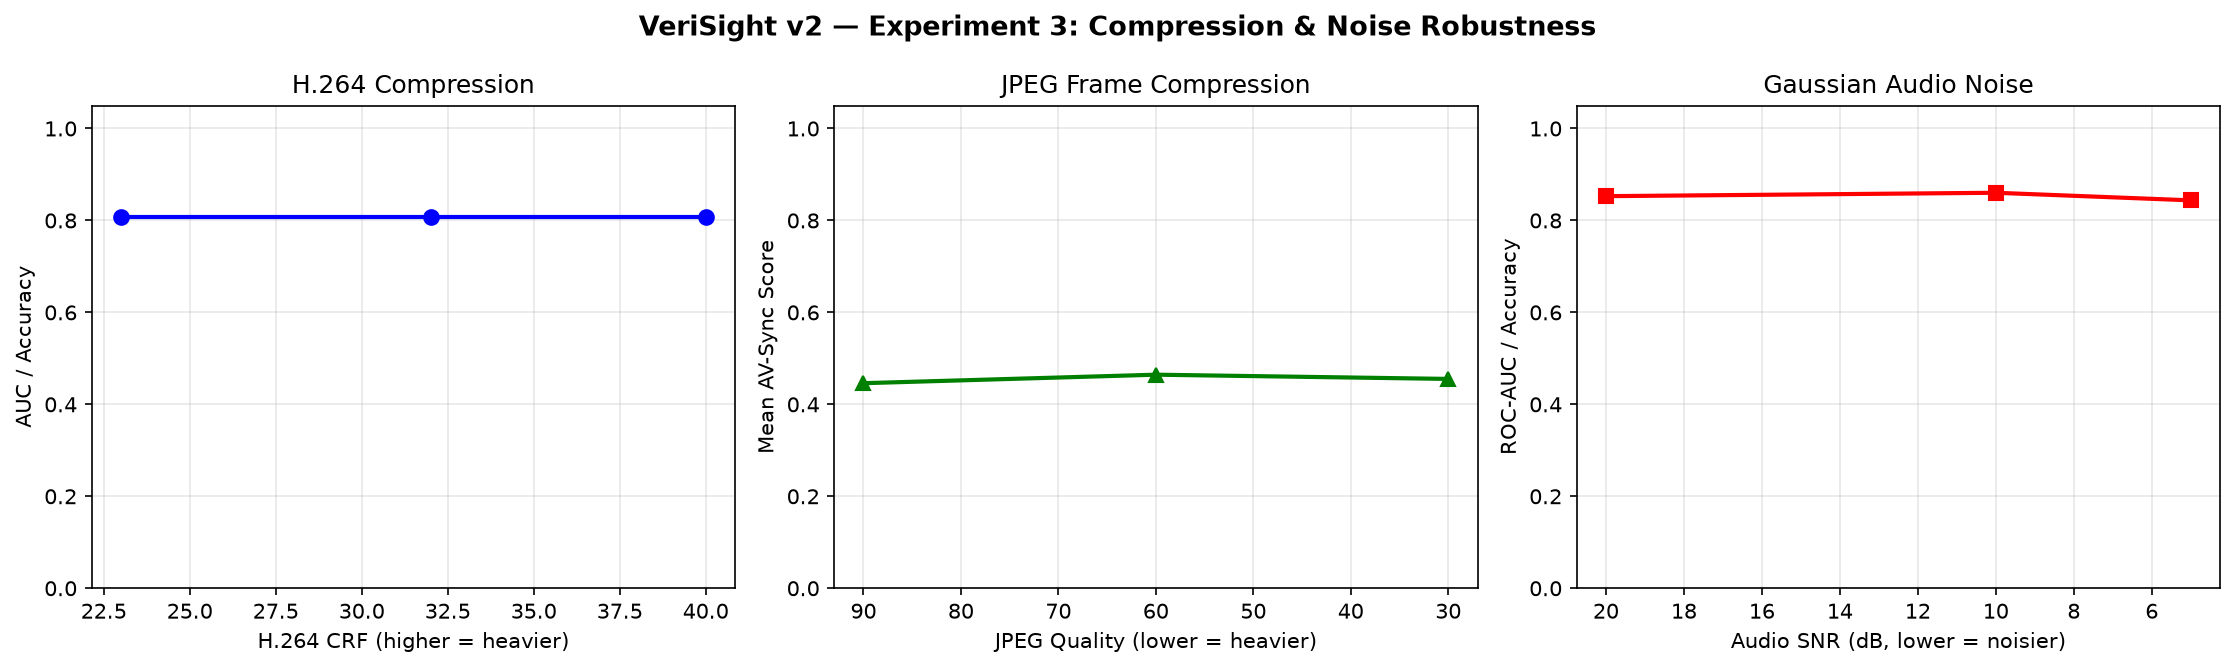
\includegraphics[width=\linewidth]{results/plots/exp3_compression_curves.png}
\caption{Experiment 3 compression and noise stress curves across H.264 CRF (23/32/40), JPEG quality (90/60/30), and Gaussian audio SNR (20/10/5\,dB).}
\label{fig:exp3_comp}
\end{figure}

\begin{figure}[htbp]
\centering
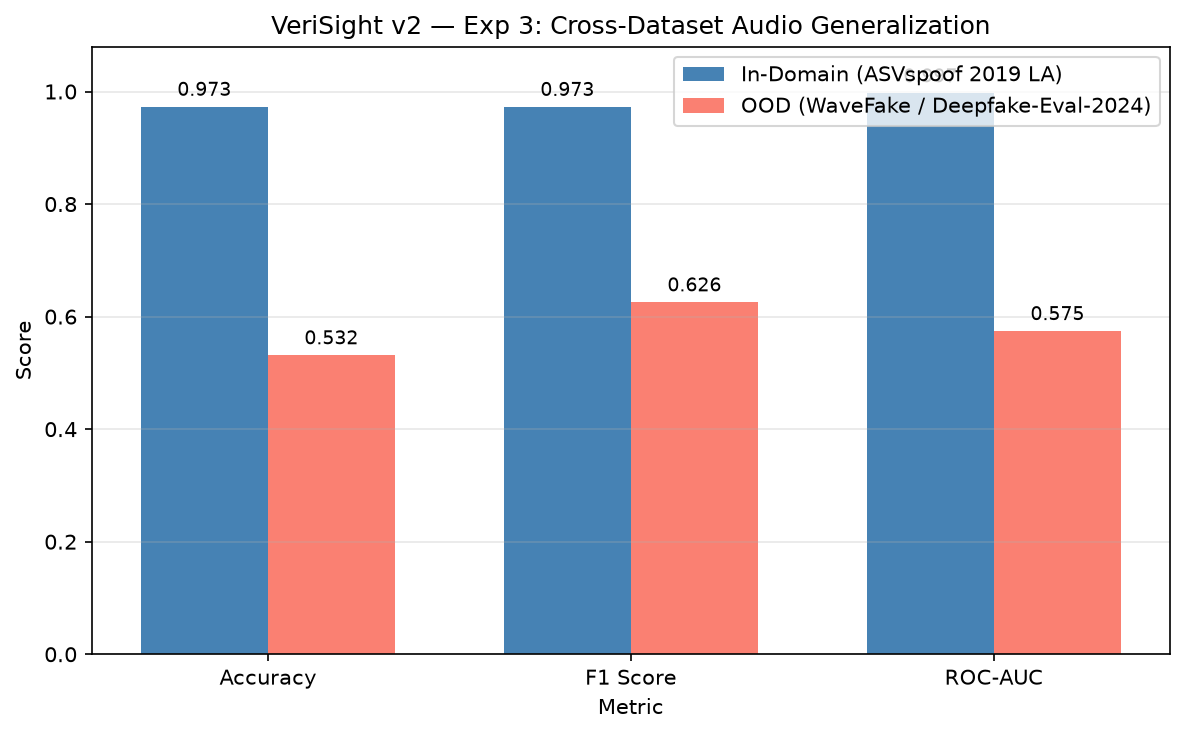
\includegraphics[width=\linewidth]{results/plots/exp3_audio_cross_dataset.png}
\caption{Audio generalization gap between in-domain ASVspoof 2019 LA (0.9972 AUC) and unseen out-of-domain neural speech (0.5747 AUC).}
\label{fig:exp3_ood}
\end{figure}

Under Experiment~3 stress testing (Table~\ref{tab:stress}, Fig.~\ref{fig:exp3_comp}), audio AUC stays stable across 20\,dB, 10\,dB, and 5\,dB Gaussian noise, while H.264 compression across CRF 23, 32, and 40 holds steady at 0.8075 AUC. Fig.~\ref{fig:exp3_ood} exposes the core limitation of unimodal audio detection: accuracy drops from 97.33\% on ASVspoof 2019 LA to 53.17\% on OOD samples (0.5747 ROC-AUC), explaining why commercial 2026 neural voices evade standalone acoustic models and validating our multimodal design. Live end-to-end API tests verified all endpoints (\texttt{200 OK}): synthetic audio demo (\texttt{0.8782 FAKE}), video face-swap demo (\texttt{vis=0.9243, aud=0.9410}), real portraits (\texttt{0.4205--0.4275 REAL}), Hindi weather (\texttt{0.2293 REAL}), Hinglish scams (\texttt{0.9757 FAKE}), and typo-heavy English (\texttt{0.2119 REAL}).

\section{Conclusion and Future Work}
VeriSight combines lightweight domain-adapted encoders, explicit cross-modal contradiction checks, and calibrated three-way abstention into a deployable verification system across English, Hindi, Hinglish, images, audio, and video. Future iterations should incorporate modern commercial neural TTS codecs (e.g., ElevenLabs) into audio training, fine-tune diffusion detectors on non-photographic vector diagrams, and replace 8-frame sampling with temporal video attention on cloud GPUs.

\begin{thebibliography}{20}
\bibitem{b1} Z. Zhang et al., ``FakeShield: Explainable image forgery detection and localization via multi-modal large language models,'' in \textit{Proc. ICLR}, 2025.
\bibitem{b2} X. Liu et al., ``MMFakeBench: A mixed-source multimodal misinformation detection benchmark,'' in \textit{Proc. ICLR}, 2025.
\bibitem{b3} N. Chandra et al., ``Deepfake-Eval-2024: A multi-modal in-the-wild benchmark of deepfakes,'' \textit{arXiv preprint}, 2025.
\bibitem{b4} Z. Cai et al., ``AV-Deepfake1M: A large-scale LLM-driven audio-visual deepfake dataset,'' in \textit{Proc. ACM MM}, 2024.
\bibitem{b5} T. Oorloff et al., ``AVFF: Audio-visual feature fusion for video deepfake detection,'' in \textit{Proc. CVPR}, 2024.
\bibitem{b6} D. Cozzolino et al., ``Raising the bar of AI-generated image detection with CLIP,'' in \textit{Proc. CVPRW}, 2024.
\bibitem{b7} W. Yang et al., ``AVoiD-DF: Audio-visual joint learning for detecting deepfake,'' \textit{IEEE Trans. Inf. Forensics Security}, 2023.
\bibitem{b8} U. Ojha et al., ``Towards universal fake image detectors that generalize across generative models,'' in \textit{Proc. CVPR}, 2023.
\bibitem{b9} Y. Chen et al., ``Cross-modal ambiguity learning for multimodal fake news detection (CAFE),'' in \textit{Proc. WWW}, 2022.
\bibitem{b10} J.-w. Jung et al., ``AASIST: Audio anti-spoofing using integrated spectro-temporal graph attention networks,'' in \textit{Proc. ICASSP}, 2022.
\bibitem{b11} N. M. M\"uller et al., ``Does audio deepfake detection generalize?'' in \textit{Proc. Interspeech}, 2022.
\bibitem{b12} H. Khalid et al., ``FakeAVCeleb: A novel audio-video multimodal deepfake dataset,'' in \textit{Proc. NeurIPS Datasets and Benchmarks}, 2021.
\bibitem{b13} A. Haliassos et al., ``Lips don't lie: A generalisable and robust approach to face forgery detection,'' in \textit{Proc. CVPR}, 2021.
\bibitem{b14} Y. Wu et al., ``Multimodal fusion with co-attention networks for fake news detection (MCAN),'' in \textit{Findings of ACL}, 2021.
\bibitem{b15} Y. Li et al., ``Celeb-DF: A large-scale challenging dataset for deepfake forensics,'' in \textit{Proc. CVPR}, 2020.
\bibitem{b16} K. Nakamura, S. Levy, and W. Y. Wang, ``r/Fakeddit: A new multimodal benchmark dataset for fine-grained fake news detection,'' in \textit{Proc. LREC}, 2020.
\bibitem{b17} A. R\"ossler et al., ``FaceForensics++: Learning to detect manipulated facial images,'' in \textit{Proc. ICCV}, 2019.
\bibitem{b18} L. Li et al., ``Face X-Ray for more general face forgery detection,'' in \textit{Proc. CVPR}, 2020.
\bibitem{b19} K. Shiohara and T. Yamasaki, ``Detecting deepfakes with self-blended images,'' in \textit{Proc. CVPR}, 2022.
\bibitem{b20} B. Dolhansky et al., ``The DeepFake Detection Challenge (DFDC) dataset,'' \textit{arXiv preprint}, 2020.
\end{thebibliography}

\end{document}
